\documentclass[11pt]{article}
\usepackage[T1]{fontenc}
\usepackage[utf8]{inputenc}
\usepackage{lmodern}
\usepackage[margin=1in]{geometry}
\usepackage{amsmath,amssymb,amsthm,mathtools}
\usepackage{microtype}
\usepackage[dvipsnames]{xcolor}
\usepackage{tikz}
\usepackage[colorlinks=true,linkcolor=MidnightBlue,citecolor=MidnightBlue,urlcolor=MidnightBlue]{hyperref}
\pdfinfoomitdate=1
\pdftrailerid{}
\pdfsuppressptexinfo=15
\newtheorem{theorem}{Theorem}[section]
\newtheorem{proposition}[theorem]{Proposition}
\newtheorem{lemma}[theorem]{Lemma}
\newtheorem{corollary}[theorem]{Corollary}
\theoremstyle{remark}
\newtheorem{remark}[theorem]{Remark}
\numberwithin{equation}{section}
\title{A Three-Manifold Without Conjugate Points and Without a Nonpositively Curved Metric}
\author{OpenAI}
\date{September 24, 2026}
\hypersetup{pdftitle={A Three-Manifold Without Conjugate Points and Without a Nonpositively Curved Metric},pdfauthor={OpenAI}}
\begin{document}
\maketitle
\begin{abstract}
We construct a closed connected orientable smooth three-manifold that admits a smooth Riemannian metric without conjugate points but admits no smooth Riemannian metric of nonpositive sectional curvature.
\end{abstract}
\tableofcontents
\section{Introduction}

A Riemannian metric has \emph{no conjugate points} if no nonzero Jacobi
field along a geodesic vanishes at two distinct times. Nonpositive
sectional curvature implies this condition. Gulliver showed that the
converse fails for an individual metric: local modifications of negatively
curved metrics can produce regions of positive curvature while preserving
the absence of conjugate points \cite[Section~3]{Gulliver1975}. Those
examples retain a manifold that already admits a negatively curved
metric. The existence question is therefore different: must a closed
manifold carrying a metric without conjugate points also carry some
metric of nonpositive sectional curvature?

This question appears in Ivanov and Kapovitch
\cite[Questions~1.1 and~8.1]{IvanovKapovitch2014} and in the survey of
Burns and Matveev \cite[Question~4.1.2]{BurnsMatveev2021}, which explicitly
includes dimension three. A closed surface without conjugate points
has universal cover diffeomorphic to $\mathbb R^2$ by the exponential
map, and hence has nonpositive Euler characteristic. Uniformization
then supplies a flat or negatively curved metric, so the existence
problem begins in dimension three. Ivanov and Kapovitch identify graph manifolds
as a central three-dimensional test case and ask about gluings of two
punctured-torus products \cite[Section~8]{IvanovKapovitch2014}.
We give a negative answer in dimension three, using a metric on a
two-piece graph manifold whose topology obstructs nonpositive curvature.

\begin{theorem}\label{thm:main}
There exists a closed connected orientable smooth three-manifold $M$ with a $C^\infty$ Riemannian metric without conjugate points, such that $M$ admits no $C^\infty$ Riemannian metric whose sectional curvature is everywhere at most zero.
\end{theorem}

The obstruction is stronger than the Riemannian assertion in the theorem.
The group $\pi_1(M)$ admits no proper cocompact isometric action on a
nonempty proper $\operatorname{CAT}(0)$ space
(Theorem~\ref{thm:no-cat0-action}); consequently, $M$ admits no locally
$\operatorname{CAT}(0)$ length metric inducing its topology
(Corollary~\ref{cor:no-local-cat0}).

The same manifold also admits no metric without focal points.
Recall that a metric has \emph{no focal points} if, for every nonzero
normal Jacobi field $J$ along a unit-speed geodesic with $J(0)=0$,
one has $\frac{d}{ds}|J(s)|^2>0$ for $s>0$. This condition is stronger
than absence of conjugate points. Ivanov and Kapovitch prove that a
closed three-manifold admits a metric without focal points if and only
if it admits a metric of nonpositive sectional curvature
\cite[Theorem~7.1]{IvanovKapovitch2014}. Their equivalence and
Theorem~\ref{thm:main} give the stated additional obstruction.

The manifold is obtained by gluing two copies of $\Sigma\times S^1$,
where $\Sigma$ is a compact oriented surface of genus one with one
boundary component. Write $h_i$ for the surface boundary and $f_i$ for
the circle factor in the $i$th boundary torus. The gluing is
\[
 h_2=h_1+f_1,\qquad f_2=h_1.
\]
This is an instance of Leeb's two-piece graph-manifold obstruction
\cite[Section~4.1, Example~4.1]{Leeb1995}. We include the group-theoretic
proof, which also gives the stronger action obstruction above.
Under a hypothetical nonpositively curved metric, the common torus
group acts by translations on a Euclidean plane. In each product piece,
the surface boundary is a commutator of elements commuting with the
fiber. The resulting translation vectors must be perpendicular.
These two orthogonality conditions are incompatible with the gluing.

The main work is the metric construction and its geodesic estimate.
Each product piece has nonpositive sectional curvature. Between them
we insert a neck $[0,1]\times T^2$ with metric
\[
 g=dt^2+dx^{\mathsf T}P(t)^{-1}\,dx,
\]
where $P(t)$ is a smooth path of positive definite matrices. We call
$P$ the \emph{cometric}, since it is the inverse torus metric. We choose
it concave, meaning that $-P''$ is positive semidefinite, with exact
product formulas near the ends. A small parameter $\delta$ controls
its derivatives; a shear of size $\delta^2$ realizes the integral
gluing after the torus periods are chosen. Convex warped collars then
join the endpoints smoothly to punctured-torus cores.

For the absence of conjugate points, we use the classical index-form
framework \cite[Sections~13--15]{Milnor1963}. Concavity of $P$ makes
the coordinate second variation nonnegative, but the intrinsic index
form differs by endpoint terms. The estimates must allow arbitrary
field values at the ends of an entire neck passage, so that they can
be combined with the estimates in the product pieces. A tangential
change of field handles passages with no turn. A returning geodesic
requires an estimate over its whole excursion.

For such an excursion, a positive boundary term controls one component
of the endpoint change in the torus part of the variation field.
We combine this control with the coordinate energy by Hilbert-space
Cauchy--Schwarz and a quadratic minimization. A strict timing margin
for excursions leaving an endpoint collar makes the estimate uniform
in the entry angle, turning height, and excursion time. No upper
bound on the duration is needed. This is what permits one metric to
handle every complete geodesic.

Section~\ref{sec:topology} fixes the manifold and proves its curvature
obstruction. Section~\ref{sec:cometric} constructs the metric and
establishes the matrix estimates. Section~\ref{sec:variations} derives
the index identities and classifies neck passages, and
Section~\ref{sec:turning} proves the returning-passage estimate.
Section~\ref{sec:global} sums the intrinsic index integrals of the
original field over all visits, including infinitely many visits,
and completes the proof of Theorem~\ref{thm:main}.
Appendix~\ref{app:punctured-torus} records the hyperbolic cusp model
used for the compact product cores.

\section{The manifold and the obstruction to nonpositive curvature}
\label{sec:topology}

We first choose the underlying manifold.  Its two product pieces impose
incompatible orthogonality conditions on the gluing torus under any
nonpositively curved metric.  This is an instance of Leeb's two-piece graph-manifold
obstruction \cite[Section~4.1, Example~4.1]{Leeb1995}.  The obstruction to
proper cocompact actions on proper CAT(0) spaces is also contained in the
group-theoretic framework of Kapovich and Leeb
\cite[Theorem~2.4]{KapovichLeeb1996}.  We give the group-theoretic argument
explicitly, since it fixes the gluing convention used in the metric construction.

\subsection{Two product pieces and one shear}

Let $\Sigma$ be a compact connected oriented surface of genus one with one
boundary component, and let $N_i=\Sigma\times S^1$ for $i=1,2$.
On $\partial N_i$ write $h_i$ for the oriented boundary circle of $\Sigma$
and $f_i$ for the positively oriented circle factor.  Thus $(h_i,f_i)$ is
an oriented integral basis of $\pi_1(\partial N_i)\cong\mathbb Z^2$.
Choose the linear diffeomorphism $\varphi:\partial N_2\longrightarrow
\partial N_1$ whose action on these bases is
\begin{equation}\label{eq:torus-gluing}
 h_2=h_1+f_1,\qquad f_2=h_1.
\end{equation}
Here and below additive notation is used only inside the torus group.
The matrix of $\varphi_*$ is
$\left(\begin{smallmatrix}1&1\\1&0\end{smallmatrix}\right)$, with determinant
$-1$, so $\varphi$ reverses the induced boundary orientations.
Gluing the two pieces by $\varphi$ therefore gives a closed connected
oriented smooth three-manifold $M$.  More explicitly, collar coordinates
give smooth charts across the identified boundary; the compact pieces
cover $M$, every boundary component is paired, and the common torus makes
the union connected.  We insert a product cylinder $[0,1]\times T^2$
between the two pieces.  Inserting this collar leaves the diffeomorphism
type unchanged and provides the region where the metric will vary.

The coordinate realization needed later is worth recording.  For any
$\epsilon>0$ and $B_2>0$, put $B_1=\epsilon B_2$ and
\[
 T^2=\mathbb R^2/\Lambda,\qquad
 \Lambda=\mathbb Z B_1e_1+\mathbb Z B_2e_2,
\]
where $e_1,e_2$ are the standard coordinate vectors.  At the first end use
the frame $(e_1,e_2)$ with respective coordinate periods $(B_1,B_2)$.
At the second end use the frame $(e_2+\epsilon e_1,e_1)$ with respective
periods $(B_2,B_1)$.  The first vector in each frame is the surface-boundary
direction and the second is the fiber direction.  Their period vectors are
\begin{equation}\label{eq:torus-periods}
 \begin{aligned}
 h_1&: B_1e_1,& f_1&:B_2e_2,\\
 h_2&:B_2(e_2+\epsilon e_1)=B_1e_1+B_2e_2,
 &f_2&:B_1e_1.
 \end{aligned}
\end{equation}
In particular the second pair is a basis of exactly the same lattice,
and these physical periods implement \eqref{eq:torus-gluing}.

Choose basepoints and connecting paths through the cylinder so that the
boundary groups are identified by \eqref{eq:torus-gluing}.  For suitable
free generators $a_i,b_i$ of $\pi_1(\Sigma)$, the boundary element is
$h_i=[a_i,b_i]^{\pm1}$.  This cyclically reduced nonempty word has infinite
order in the free group.  Consequently
\[
 G_i:=\pi_1(N_i)=F(a_i,b_i)\times\langle f_i\rangle,
 \qquad
 \langle h_i,f_i\rangle\cong\mathbb Z^2
\]
and the boundary-group inclusion in each $G_i$ is injective: a relation
$h_i^m f_i^n=1$ first gives $n=0$ by projection onto the circle factor
and then $m=0$ in the free group.  Van Kampen's theorem and the normal form
for an amalgamated product give
\begin{equation}\label{eq:amalgam}
 \Gamma:=\pi_1(M)=G_1*_{\Gamma_T}G_2,
 \qquad \Gamma_T=\langle h_1,f_1\rangle=\langle h_2,f_2\rangle\cong\mathbb Z^2,
\end{equation}
with both vertex groups and $\Gamma_T$ embedded in $\Gamma$.
For $f\in\Gamma$, write
$C_\Gamma(f)=\{g\in\Gamma:gf=fg\}$ for its centralizer.  Since $f_i$ is
central in $G_i$, we have
\begin{equation}\label{eq:boundary-commutators}
 G_i\subset C_\Gamma(f_i),\qquad
 h_i\in[C_\Gamma(f_i),C_\Gamma(f_i)]\quad(i=1,2).
\end{equation}

\subsection{The two incompatible orthogonality conditions}

\begin{theorem}\label{thm:no-cat0-action}
The fundamental group $\Gamma=\pi_1(M)$ of the closed three-manifold
defined by \eqref{eq:torus-gluing} admits no proper cocompact isometric
action on a nonempty proper $\operatorname{CAT}(0)$ space.
\end{theorem}

\begin{proof}
Suppose that $\Gamma$ acts properly and cocompactly by isometries on a
nonempty proper $\operatorname{CAT}(0)$ space $X$.  Properness of the action
means that for compact sets $K,L\subset X$, only finitely many
$g\in\Gamma$ satisfy $gK\cap L\ne\varnothing$; in particular, point
stabilizers are finite.

For $g\in\Gamma$ set
\[
 \ell(g)=\inf_{x\in X}d(x,gx),\qquad
 \operatorname{Min}(g)=\{x\in X:d(x,gx)=\ell(g)\}.
\]
We check the attainment of this infimum before applying the flat torus
theorem.  Choose $x_n$ with $d(x_n,gx_n)\to\ell(g)$ and a compact set
$K\subset X$ whose $\Gamma$-translates cover $X$.  There are $k_n\in\Gamma$
such that $y_n=k_nx_n\in K$.  Put $g_n=k_ngk_n^{-1}$.
For all large $n$, $d(y_n,g_ny_n)\le\ell(g)+1$.  The closed
$(\ell(g)+1)$-neighborhood of $K$ is compact, because $X$ is proper.
Properness of the action therefore permits only finitely many $g_n$.
After passage to a subsequence, $g_n=g_*$ and $y_n\to y\in K$, whence
$d(y,g_*y)=\ell(g)$.  Since translation length is invariant under
conjugation, conjugating $y$ back gives a point of
$\operatorname{Min}(g)$.  Thus every element of $\Gamma$ is semisimple.
If $g$ has infinite order, its attained minimum is positive: otherwise
$g$ fixes a point, and its infinitely many distinct powers belong to that
point stabilizer, contrary to its finiteness.  The semisimplicity argument
is also given in
\cite[Proposition~II.6.10(2)]{BridsonHaefliger1999}.

Apply the flat torus theorem
\cite[Theorem~II.7.1(1)--(3)]{BridsonHaefliger1999} to the embedded group
$\Gamma_T\cong\mathbb Z^2$.  Its action is proper and semisimple by the preceding
paragraph.  Hence
\[
 \operatorname{Min}(\Gamma_T):=\bigcap_{a\in\Gamma_T}\operatorname{Min}(a)
       \cong Y\times\mathbb R^2,
\]
and $\Gamma_T$ acts trivially on $Y$ and as a translation lattice on
$\mathbb R^2$.  Fix one of these invariant Euclidean planes, denoted $E$,
and write $\mathbf v(a)\in\mathbb R^2$ for the translation vector of
$a\in\Gamma_T$.  The map $\mathbf v$ is a homomorphism, and its values on any
integral basis of $\Gamma_T$ are linearly independent.

We now use the boundary-commutator relation
\eqref{eq:boundary-commutators}.  For each $i$, the positive translation
length $\ell_i=\ell(f_i)$ and the cyclic minset theorem give
\begin{equation}\label{eq:cyclic-minset}
 \operatorname{Min}(f_i)\cong Y_i\times\mathbb R,
 \qquad f_i(y,t)=(y,t+\ell_i).
\end{equation}
Every $g\in C_\Gamma(f_i)$ preserves this product and acts as
\[
 g(y,t)=(g_i'(y),t+\tau_i(g)),
\]
where $\tau_i(g)$ is a real number independent of $y$;
see \cite[Theorem~II.6.8(4)--(5)]{BridsonHaefliger1999}.
To see the reason for this product action, commutation sends each oriented
$f_i$-axis to another such axis.  In the splitting
\eqref{eq:cyclic-minset}, these are the lines $\{y\}\times\mathbb R$.
An axiswise translation could initially have a shift depending on $y$,
but preservation of the product distance between $(y,t)$ and $(z,s)$
for every $t-s\in\mathbb R$ forces the two shifts to agree.
Composition now shows that
$\tau_i:C_\Gamma(f_i)\longrightarrow(\mathbb R,+)$ is a homomorphism.
It vanishes on commutators, so $\tau_i(h_i)=0$.

The same plane $E$ lies in both cyclic minsets, because
$E\subset\operatorname{Min}(\Gamma_T)$.  At a point $x=(y,t)\in E$ expressed
in the $i$th splitting, the zero shift of $h_i$ gives
\[
 \begin{aligned}
 d(x,h_if_ix)^2
 &=d_{Y_i}(y,h_i'y)^2+\ell_i^2\\
 &=d(x,h_ix)^2+d(x,f_ix)^2.
 \end{aligned}
\]
All three distances can also be computed in the Euclidean plane $E$.
It follows that
\begin{equation}\label{eq:torus-orthogonality}
 \langle\mathbf v(h_i),\mathbf v(f_i)\rangle=0
 \qquad(i=1,2).
\end{equation}
Put $u=\mathbf v(h_1)$ and $v=\mathbf v(f_1)$.
The first equality in \eqref{eq:torus-orthogonality} says
$\langle u,v\rangle=0$.  The gluing relations give
$\mathbf v(h_2)=u+v$ and $\mathbf v(f_2)=u$, so the second equality says
\[
 0=\langle u+v,u\rangle=|u|^2.
\]
This is impossible: $h_1$ is nontrivial in $\Gamma_T$, and its translation vector
in the lattice is nonzero.
\end{proof}

\begin{corollary}\label{cor:no-local-cat0}
The manifold $M$ admits no locally $\operatorname{CAT}(0)$ length metric
inducing its manifold topology.
\end{corollary}

\begin{proof}
Suppose that such a metric exists.  Compactness of $M$ makes it complete
and locally compact.  Its ordinary universal cover, equipped with the
lifted length metric, is complete and locally compact, and the covering
map is a local isometry.  Metric Cartan--Hadamard makes this universal
cover a $\operatorname{CAT}(0)$ space, and metric Hopf--Rinow makes it
proper; see \cite[Proposition~I.3.7(1) and Theorem~II.4.1(2)]{BridsonHaefliger1999}.
The deck group $\Gamma$ acts freely and properly by isometries, with
compact quotient $M$.  This contradicts Theorem~\ref{thm:no-cat0-action}.
\end{proof}

\begin{proposition}\label{prop:no-npc}
The closed smooth three-manifold $M$ defined by
\eqref{eq:torus-gluing} admits no smooth Riemannian metric of nonpositive
sectional curvature.
\end{proposition}

\begin{proof}
Such a Riemannian metric is a length metric inducing the manifold topology
and is locally $\operatorname{CAT}(0)$
\cite[Theorem~II.1A.6]{BridsonHaefliger1999}, contradicting
Corollary~\ref{cor:no-local-cat0}.
\end{proof}

These obstructions depend only on the topology of $M$.  The metric
constructed below will have no conjugate points.

\section{A concave cometric and smooth product cores}
\label{sec:cometric}

We construct the metric in two stages.  First we join the two product
structures by a metric on the torus neck.  Then we extend its endpoint
formulas over compact punctured-torus products.  The neck estimates will
depend on a small parameter $\delta$, while the torus periods will be
chosen afterward to fit the surface boundaries into hyperbolic cusps.

\subsection{The matrix path and its endpoint coordinates}

Write $e_1,e_2$ for the standard basis of $\mathbb R^2$.
The two product structures require different diagonal coordinate frames:
$(e_1,e_2)$ on the left and $(e_2+\epsilon e_1,e_1)$ on the right.
To arrange concavity, we start with a diagonal path and introduce the
shear only where both diagonal coefficients have strictly negative
second derivative.  The diagonal variation has size $\delta$;
taking $\epsilon=\delta^2$ makes the frame change a smaller perturbation.
The periods $B_1=\epsilon B_2$ then turn this small coordinate shear into
the fixed integral gluing of Section~\ref{sec:topology}.

Define the
smooth function $a:\mathbb R\to[0,1)$ and its primitive $A$ by
\begin{equation}\label{eq:cometric-cutoff}
 a(u)=\begin{cases}
       \exp\bigl(-1/(2/3-u)\bigr),&u<2/3,\\
       0,&u\ge 2/3,
      \end{cases}
 \qquad A(u)=\int_0^u a(y)\,dy.
\end{equation}
The definition includes negative $u$, which will be needed when extending
the metric into the product pieces.  Fix once and for all a smooth
nondecreasing function $\chi:\mathbb R\to[0,1]$ equal to zero on
$(-\infty,5/12]$ and to one on $[7/12,\infty)$.
For $0<\delta\le 1/2$, set $\epsilon=\delta^2$ and define
\begin{align}
 H(t)&=e_2+\epsilon\chi(t)e_1,\notag\\
 d_1(t)&=1+\delta A(t),\qquad
 d_2(t)=1+\delta A(1-t),\notag\\
 P(t)&=d_1(t)e_1e_1^{\mathsf T}+d_2(t)H(t)H(t)^{\mathsf T},
 \qquad 0\le t\le1.
 \label{eq:cometric-path}
\end{align}
Here a superscript $\mathsf T$ denotes transpose.  For a positive definite
matrix $P$, its inverse $Q=P^{-1}$ is the matrix of the torus metric;
we therefore call $P$ the cometric.

Choose $B_2>0$ later and put $B_1=\epsilon B_2$.  On
\[
 T^2=\mathbb R^2/\Lambda,\qquad
 \Lambda=\mathbb Z B_1e_1+\mathbb Z B_2e_2,
\]
use the neck metric
\begin{equation}\label{eq:neck-metric}
 g=dt^2+dx^{\mathsf T}Q(t)\,dx.
\end{equation}
The product coordinates at the two ends are given by the frames
\begin{equation}\label{eq:end-frames}
 T_1=(e_1,e_2),\qquad T_2=(e_2+\epsilon e_1,e_1),\qquad x=T_i y.
\end{equation}
At the first end the two coordinate periods are $B_1,B_2$; at the second
they are $B_2,B_1$. The first coordinate is the surface-boundary direction
and the second is the circle factor. The period calculation
\eqref{eq:torus-periods} shows that these frames give exactly the gluing
\eqref{eq:torus-gluing}.

Let $\tau=t$ at the first end and $\tau=1-t$ at the second, so that
$\tau$ increases into the neck.  A constant coordinate change $x=T_i y$
changes the cometric by $P\mapsto T_i^{-1}PT_i^{-\mathsf T}$.
Since $A$ is constant on $[2/3,\infty)$, in these endpoint coordinates
we have the exact identities
\begin{equation}\label{eq:end-cometric}
 P_i(\tau)=\begin{pmatrix}1+\delta A(\tau)&0\\0&b\end{pmatrix},
 \qquad b=1+\delta A(1),\qquad 0\le\tau\le1/4.
\end{equation}
In particular
\begin{equation}\label{eq:end-cometric-slope}
 P_i(0)e_1=e_1,
 \qquad P_i'(0)=\kappa e_1e_1^{\mathsf T},
 \qquad \kappa=\delta a(0)>0.
\end{equation}
Primes on $P_i$ refer to $\tau$.

For symmetric matrices $R,S$, write $R\preceq S$ when $S-R$ is
positive semidefinite; $R\succeq S$ has the reversed meaning.

\begin{lemma}\label{lem:cometric-bounds}
There are constants $\delta_0>0$ and $C<\infty$, depending only on the
fixed function $\chi$, such that for $0<\delta\le\delta_0$ the path
\eqref{eq:cometric-path} satisfies, in the original coordinates and in
either endpoint coordinate system,
\begin{gather}
 \frac19\operatorname{Id}\preceq P\preceq18\operatorname{Id},
 \qquad
 \frac1{18}\operatorname{Id}\preceq Q\preceq9\operatorname{Id},
 \qquad \|P'\|\le C\delta,
 \label{eq:cometric-uniform}\\
 -P''\succeq0,
 \qquad |P'p|^2\le C\delta\,p^{\mathsf T}(-P'')p
 \quad\text{for every }p\in\mathbb R^2.
 \label{eq:cometric-domination}
\end{gather}
The constants do not depend on $B_1$ or $B_2$.
\end{lemma}

\begin{proof}
All matrix norms are Euclidean operator norms.
On $[0,1]$ we have $1\le d_i\le2$.  The matrix
$R=(e_1,H)$ and its inverse have squared norms at most $3$.
As $P=R\operatorname{diag}(d_1,d_2)R^{\mathsf T}$, this gives
$\operatorname{Id}/3\preceq P\preceq6\operatorname{Id}$ in the original
coordinates.  The same bounds on $\|T_i\|^2$ and $\|T_i^{-1}\|^2$
give the displayed weaker bounds in both endpoint frames.

For $u<2/3$,
\begin{equation}\label{eq:cutoff-differential}
 a'(u)=-\frac{a(u)}{(2/3-u)^2}.
\end{equation}
Consequently, on $[0,1]$,
$a^2\le-a'$ and $|a'|\le1$, with both sides zero on the plateau when
appropriate.  Put $I_0=[5/12,7/12]$.
Outside $I_0$, the vector $H$ is constant.  If $q=R^{\mathsf T}p$,
then
\[
 p^{\mathsf T}(-P'')p
 =\delta\bigl(-a'(t)q_1^2-a'(1-t)q_2^2\bigr),
\]
and
\[
 |P'p|^2
 \le3\delta^2\bigl(a(t)^2q_1^2+a(1-t)^2q_2^2\bigr)
 \le3\delta\,p^{\mathsf T}(-P'')p.
\]
This proves concavity and the required domination there, including the
directions in which $-P''$ vanishes.

On $I_0$ both $t$ and $1-t$ lie in $[5/12,7/12]$, and
\[
 -a'(t),\ -a'(1-t)\ge m,\qquad m=144e^{-12}>0.
\]
To control every error caused by the moving frame, compare $P$ with
$P_0=\operatorname{diag}(d_1,d_2)$ and write $E=P-P_0$.
The derivatives are
\begin{align*}
 P'={}&\delta a(t)e_1e_1^{\mathsf T}
       -\delta a(1-t)HH^{\mathsf T}
       +d_2\epsilon\chi'(e_1H^{\mathsf T}+He_1^{\mathsf T}),\\
 P''={}&\delta a'(t)e_1e_1^{\mathsf T}
       +\delta a'(1-t)HH^{\mathsf T}
       -2\delta a(1-t)\epsilon\chi'
              (e_1H^{\mathsf T}+He_1^{\mathsf T})\\
       &+d_2\epsilon\chi''(e_1H^{\mathsf T}+He_1^{\mathsf T})
       +2d_2\epsilon^2(\chi')^2e_1e_1^{\mathsf T}.
\end{align*}
Using $|H|\le\sqrt2$ and
$\|HH^{\mathsf T}-e_2e_2^{\mathsf T}\|\le3\epsilon$ gives
\[
 \|E'\|\le C_1\epsilon,
 \qquad \|E''\|\le C_2\epsilon,
\]
where $C_1,C_2$ depend only on the fixed function $\chi$.
These estimates use only $\delta,\epsilon\le1$ and $d_2\le2$.
Take
$\delta_0\le\min\{1/2,m/(2C_2)\}$.
Since $\epsilon=\delta^2$ and $-P_0''\succeq m\delta\operatorname{Id}$,
we obtain
\[
 -P''\succeq\tfrac12m\delta\operatorname{Id},
 \qquad \|P'\|\le(1+C_1)\delta
 \quad\text{on }I_0.
\]
It follows that
\[
 |P'p|^2\le\frac{2(1+C_1)^2}{m}\,
              \delta\,p^{\mathsf T}(-P'')p.
\]
The displayed derivative formula also gives $\|P'\|\le C\delta$
outside $I_0$.

Finally, under $\widetilde P=T_i^{-1}PT_i^{-\mathsf T}$, with
$q=T_i^{-\mathsf T}p$, the domination estimate transforms as
\[
 |\widetilde P'p|^2
 \le\|T_i^{-1}\|^2|P'q|^2
 \le3C\delta\,p^{\mathsf T}(-\widetilde P'')p.
\]
Reversing $t$ at the second end changes the sign of the first derivative
and leaves the second derivative unchanged.  This proves all assertions.
\end{proof}

\subsection{Smooth convex collars}

The endpoint metric in \eqref{eq:end-cometric} is the product of a flat
circle and the surface metric
\[
 d\tau^2+\ell_0(\tau)^2dy_1^2,
 \qquad \ell_0(\tau)=(1+\delta A(\tau))^{-1/2}.
\]
Its Gaussian curvature is $-\ell_0''/\ell_0$.  Direct differentiation
gives
\begin{equation}\label{eq:end-warp-convexity}
 \frac{\ell_0''}{\ell_0}
 =\frac{3\delta^2a^2}{4(1+\delta A)^2}
  -\frac{\delta a'}{2(1+\delta A)}\ge0.
\end{equation}
Thus the neck already has nonpositive sectional curvature on
$0\le t\le1/4$ and $3/4\le t\le1$.
We next extend each endpoint surface metric inward to a hyperbolic cusp
by an explicit convex warping function.

For $-1\le\tau\le0$ we have $A(\tau)\ge-1$, so
$1+\delta A(\tau)\ge1/2$.  Define
\[
 r(\tau)=\frac{\delta a(\tau)}{2(1+\delta A(\tau))}.
\]
For $0<\delta\le1/2$, this is positive and at most $\delta\le1/2$;
moreover
\[
 r'(\tau)=\frac{\delta\bigl(a'(\tau)(1+\delta A(\tau))
                                  -\delta a(\tau)^2\bigr)}
                         {2(1+\delta A(\tau))^2}<0.
\]
Fix a smooth nondecreasing function $\lambda:[-1,0]\to[0,1]$ equal to
zero near $-1$ and one near $0$.  Put
\begin{equation}\label{eq:collar-warp}
 k=1-\lambda+\lambda r,
 \qquad \ell(\tau)=\exp\left(-\int_0^\tau k(u)\,du\right).
\end{equation}
Then $k>0$ and
$k'=\lambda'(r-1)+\lambda r'\le0$.  Hence
\[
 \ell''=(k^2-k')\ell>0.
\]
Near zero, $k=r$ and $\ell(0)=1$, which proves the exact equality
$\ell=(1+\delta A)^{-1/2}$ there.  Near $-1$, $k=1$, so
\begin{equation}\label{eq:collar-cusp-germ}
 \ell(\tau)=\ell(-1)e^{-(\tau+1)}.
\end{equation}
Both matching assertions hold on open collars, not only to a finite
order at their endpoints.

\subsection{Punctured-torus cores and the final gluing}

Fix a complete finite-area hyperbolic punctured torus.  It has an embedded
cusp of the form
\begin{equation}\label{eq:hyperbolic-cusp}
 dr^2+c^2e^{-2r}d\theta^2,
 \qquad r\ge0,\quad \theta\in\mathbb R/\mathbb Z,
\end{equation}
for some $c>0$.  In particular, its cusp contains a horocycle of every
sufficiently small positive length.  An explicit ideal-quadrilateral
construction, following \cite[Section~5.5]{Bonahon2009}, is recalled in
Appendix~\ref{app:punctured-torus}.

Fix $\delta$ to meet both Lemma~\ref{lem:cometric-bounds} and the
additional upper bounds imposed by the index-form estimates below.
Only after this choice, choose $B_2$ so small that both numbers
$B_i\ell(-1)$, $i=1,2$, occur as lengths of horocycles in an embedded
cusp \eqref{eq:hyperbolic-cusp}, and set $B_1=\delta^2B_2$ as above.
For each $i$, truncate a copy of the punctured torus at the horocycle
of length $B_i\ell(-1)$, retain the compact side, and attach
$[-1,0]\times(\mathbb R/B_i\mathbb Z)$ with metric
$d\tau^2+\ell(\tau)^2dy_1^2$.
To check smoothness at $\tau=-1$, if the truncation is at $r=r_i$,
set
\[
 r=r_i+\tau+1,\qquad \theta=y_1/B_i.
\]
The cusp metric becomes
$d\tau^2+\ell(-1)^2e^{-2(\tau+1)}dy_1^2$ on a neighborhood of
the seam, which agrees exactly with \eqref{eq:collar-cusp-germ}.
The resulting compact surface $\Sigma_i$ has genus one and one boundary
component, and has Gaussian curvature at most zero.

Give
$N_i=\Sigma_i\times(\mathbb R/B_{3-i}\mathbb Z)$ the product metric
with circle term $b^{-1}dy_2^2$.  The metrics on $N_i$ have nonpositive
sectional curvature.  At their remaining boundaries, their formulas
agree on full collars with \eqref{eq:end-cometric}, so the torus maps
\eqref{eq:end-frames} attach them smoothly to the neck.  The result is
a $C^\infty$ Riemannian metric on the closed connected three-manifold
specified by $h_2=h_1+f_1$, $f_2=h_1$.
Every part outside the open neck, as well as its two indicated endpoint
portions, has nonpositive sectional curvature.  Choosing the periods
after $\delta$ does not affect any estimate on the lifted neck metric.

Figure~\ref{fig:neck-gluing} records the two inward coordinates and
shows how the period relation turns the small coordinate shear into
the fixed integral gluing.
\begin{figure}[tbp]
\centering
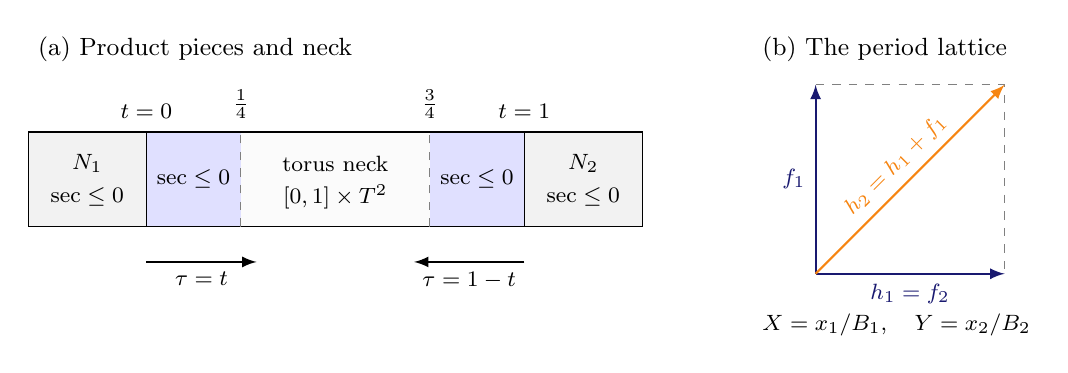
\begin{tikzpicture}[x=1cm,y=1cm,>=latex,font=\footnotesize]
  \node[anchor=west,font=\small] at (0,3.15)
    {(a) Product pieces and neck};
  \fill[gray!10] (0,0.9) rectangle (1.5,2.1);
  \fill[gray!10] (6.3,0.9) rectangle (7.8,2.1);
  \fill[Blue!12] (1.5,0.9) rectangle (2.7,2.1);
  \fill[Blue!12] (5.1,0.9) rectangle (6.3,2.1);
  \fill[gray!3] (2.7,0.9) rectangle (5.1,2.1);
  \draw (0,0.9) rectangle (7.8,2.1);
  \draw (1.5,0.9) -- (1.5,2.1);
  \draw (6.3,0.9) -- (6.3,2.1);
  \draw[dashed,gray] (2.7,0.9) -- (2.7,2.1);
  \draw[dashed,gray] (5.1,0.9) -- (5.1,2.1);
  \node at (0.75,1.7) {$N_1$};
  \node at (7.05,1.7) {$N_2$};
  \node at (0.75,1.28) {$\sec\le0$};
  \node at (7.05,1.28) {$\sec\le0$};
  \node at (2.1,1.5) {$\sec\le0$};
  \node at (5.7,1.5) {$\sec\le0$};
  \node at (3.9,1.7) {torus neck};
  \node at (3.9,1.28) {$[0,1]\times T^2$};
  \node[above] at (1.5,2.15) {$t=0$};
  \node[above] at (2.7,2.15) {$\frac14$};
  \node[above] at (5.1,2.15) {$\frac34$};
  \node[above] at (6.3,2.15) {$t=1$};
  \draw[->,thick] (1.5,0.45) -- (2.9,0.45)
    node[midway,below] {$\tau=t$};
  \draw[->,thick] (6.3,0.45) -- (4.9,0.45)
    node[midway,below] {$\tau=1-t$};

  \node[anchor=west,font=\small] at (9.2,3.15)
    {(b) The period lattice};
  \draw[dashed,gray] (10,2.7) -- (12.4,2.7) -- (12.4,0.3);
  \draw[->,thick,MidnightBlue] (10,0.3) -- (12.4,0.3)
    node[midway,below] {$h_1=f_2$};
  \draw[->,thick,MidnightBlue] (10,0.3) -- (10,2.7)
    node[midway,left] {$f_1$};
  \draw[->,thick,BurntOrange] (10,0.3) -- (12.4,2.7)
    node[midway,above,sloped] {$h_2=h_1+f_1$};
  \node[anchor=west] at (9.2,-0.35)
    {$X=x_1/B_1,\quad Y=x_2/B_2$};
\end{tikzpicture}
\caption{The construction in schematic coordinates.  Each product piece
$N_i$ includes its convex collar; the two end portions of the neck also have
nonpositive sectional curvature.  The arrows indicate the inward
coordinate at each end.  The lattice cell is drawn in normalized
coordinates $(X,Y)$: since $B_1=\epsilon B_2$, its diagonal represents
$h_2=B_2(e_2+\epsilon e_1)=h_1+f_1$ even when the coordinate shear
$\epsilon$ is small.  Physical lengths are not to scale, and drawn angles
are not angles of the Riemannian metric.}
\label{fig:neck-gluing}
\end{figure}


\section{Geodesic passages and the index form}\label{sec:variations}

We now study the index form along a complete unit-speed geodesic of the
constructed metric.  The metric outside the neck has nonpositive sectional
curvature.  Inside the neck, concavity of the inverse metric gives a nonnegative
coordinate expression for the second variation.  The distinction between
that expression and the intrinsic index form is an endpoint term.  We first
compute that term and dispose of the passages that have no turn; the next
section estimates the remaining turning passages.

Throughout this section the neck metric is
\[
 g=dt^2+dx^{\mathsf T}Q(t)\,dx,\qquad P(t)=Q(t)^{-1},\qquad 0\le t\le1,
\]
with the smooth positive definite matrices constructed above.  In particular,
$-P''(t)$ is positive semidefinite.  At either boundary, we may use its inward
coordinate $\tau$ and its fixed torus frame.  In these coordinates,
\begin{equation}\label{eq:variational-end-germ}
 P(\tau)=\operatorname{diag}(1+\delta A(\tau),b)
 \quad(0\le\tau\le1/4),\qquad
 b=1+\delta A(1),\qquad \kappa=\delta A'(0)>0.
\end{equation}
These are exactly the two frames of the construction; changing between them
is a constant linear coordinate change, together with $\tau=1-t$ at the
right boundary.  The metric and these coordinates extend smoothly through
each boundary into a product collar.  The two end portions of the neck have
nonpositive sectional curvature.

\subsection{Normal index forms and coordinate second variation}

Let $\gamma$ be a complete unit-speed geodesic, and write $T=\dot\gamma$.
For a smooth field $V$ along $\gamma$ and an interval $J$, define
\begin{align}
 I_J(V)&=\int_J\bigl(|D_sV|^2-
       \langle R(V,T)T,V\rangle\bigr)\,ds,\label{eq:index-definition}\\
 q_V&=\langle V,T\rangle,\qquad
 I_J^\perp(V)=I_J(V)-\int_J|\dot q_V|^2\,ds.
       \label{eq:normal-index-definition}
\end{align}
We use the curvature convention for which the curvature term
$\langle R(V,T)T,V\rangle$ is nonpositive when sectional curvature is
nonpositive.  When $J$ is unbounded we will only use fields vanishing for
sufficiently large $|s|$, so these integrals are finite.

\begin{lemma}[Tangential invariance]\label{lem:tangential-invariance}
The integrand defining $I_J^\perp(V)$ is the index integrand of
$V^\perp=V-q_VT$.  Consequently, for every smooth real function $h$,
\[
 I_J^\perp(V+hT)=I_J^\perp(V)
\]
provided both fields have the finite integrals required in
\eqref{eq:normal-index-definition}.  This invariance holds pointwise, without
any condition on $h$ at finite endpoints.
\end{lemma}

\begin{proof}
Since $D_sT=0$ and $\langle V^\perp,T\rangle=0$, we have
$\langle D_sV^\perp,T\rangle=0$ and
\[
 |D_sV|^2=|D_sV^\perp|^2+|\dot q_V|^2.
\]
The curvature symmetries give
$\langle R(V,T)T,V\rangle=
\langle R(V^\perp,T)T,V^\perp\rangle$.
Both assertions follow.
\end{proof}

On any connected interval where $\gamma$ lies in the neck, lift its torus
coordinate to $\mathbb R^2$.  With a dot denoting differentiation in $s$ and
a prime differentiation in $t$, the geodesic equations imply
\begin{equation}\label{eq:neck-geodesic}
 p=Q(t)\dot x\ \text{is constant},\qquad
 F(t)=p^{\mathsf T}P(t)p,\qquad
 v=\dot t,\qquad
 v^2=1-F(t),\qquad \dot v=-\tfrac12F'(t).
\end{equation}
Indeed, the Euler--Lagrange equation in the cyclic variable $x$ gives the
first identity.  Unit speed gives the fourth, and the $t$ equation is
$\ddot t=\dot x^{\mathsf T}Q'\dot x/2=-F'/2$.
The function $F$ is concave because $P''\preceq0$.

For a field $V=(w,z)$ in these coordinates, $w$ is its interval component
and $z$ its two torus components.  Write $|\xi|_Q^2=\xi^{\mathsf T}Q\xi$.
On a compact coordinate interval $[a,c]$, define
\begin{equation}\label{eq:linear-energy}
 E_{[a,c]}(V)=\int_a^c
 \left(\dot w^2+|\dot z-P'p\,w|_Q^2
                 -\tfrac12F''(t)w^2\right)\,ds.
\end{equation}
Every term in this expression is nonnegative. We use the same integral
to define $E_J(V)$ on an unbounded neck interval $J$ when the field
vanishes for sufficiently large $|s|$.

\begin{lemma}[Endpoint correction]\label{lem:coordinate-index}
For a smooth field $V=(w,z)$ on $[a,c]$,
\begin{equation}\label{eq:coordinate-index}
 I_{[a,c]}(V)=E_{[a,c]}(V)
       -\bigl[\langle T,\Gamma(V,V)\rangle\bigr]_a^c,
\end{equation}
where $\Gamma$ denotes the Christoffel symbols in the chosen product
coordinates and brackets mean final value minus initial value.
In the inward coordinates at either neck boundary, if $w=0$ at that
boundary, then
\begin{equation}\label{eq:boundary-christoffel}
 \Gamma(V,V)=\tfrac\kappa2 z_1^2\partial_\tau.
\end{equation}
Thus the endpoint contribution in \eqref{eq:coordinate-index} is
nonnegative at an entry into or exit from the open neck, provided the
interval component of the field vanishes there.
\end{lemma}

\begin{proof}
Consider the coordinate-linear variation
$(t(s)+r w(s),x(s)+r z(s))$.  Its energy is one half the integral of its
squared speed.  Differentiating twice at $r=0$ gives
\[
 \int_a^c\left(\dot w^2+\dot z^{\mathsf T}Q\dot z
   +2w\dot z^{\mathsf T}Q'\dot x
   +\tfrac12w^2\dot x^{\mathsf T}Q''\dot x\right)\,ds.
\]
The inverse-matrix identities
\[
 Q'=-QP'Q,\qquad
 Q''=2QP'QP'Q-QP''Q,
\]
together with $\dot x=Pp$, turn this expression into
$E_{[a,c]}(V)$.

For completeness, the endpoint term can be seen directly in the
intrinsic second variation.  If $W=\partial_r\alpha$ and
$U=\partial_s\alpha$ for a variation $\alpha$, the first energy derivative
is $[\langle W,U\rangle]_a^c-\int\langle W,D_sU\rangle$.
Differentiate once more at the geodesic $r=0$, commute the covariant
derivatives, and integrate the $D_s^2V$ term by parts.  The result is
\[
 \frac{d^2}{dr^2}\bigg|_{r=0}\frac12\int_a^c|U|^2\,ds
 =I_{[a,c]}(V)+[\langle T,D_rW\rangle]_a^c.
\]
For the coordinate-linear variation, its coordinate second derivative in
$r$ is zero, so $D_rW=\Gamma(V,V)$.  This proves
\eqref{eq:coordinate-index}.

The nonzero types of Christoffel symbols for this product-coordinate
metric are
\[
 \Gamma^t_{ij}=-\tfrac12Q'_{ij},\qquad
 \Gamma^i_{tj}=\Gamma^i_{jt}=\tfrac12(PQ')^i{}_j.
\]
At a boundary where $w=0$, only
$-z^{\mathsf T}Q'z\,\partial_\tau/2$ remains.  By
\eqref{eq:variational-end-germ}, $Q'(0)=-\kappa e_1e_1^{\mathsf T}$;
hence \eqref{eq:boundary-christoffel} follows.  At an initial boundary
$\dot\tau>0$ and this scalar is added in
\eqref{eq:coordinate-index}; at a final boundary $\dot\tau<0$ and it is
subtracted.  Both signs are nonnegative.
\end{proof}

\subsection{The possible passages}

A \emph{neck passage} is a connected component $J$ of
$\{s\in\mathbb R:0<t(\gamma(s))<1\}$.  The notation means the preimage
of the open neck; it does not require an interval coordinate away from
the neck.  A restricted compactly supported field may have arbitrary
values at finite endpoints of $J$.

\begin{lemma}[Passage classification]\label{lem:neck-passages}
Every finite endpoint of a neck passage is transverse to the boundary
torus.  Exactly one of the following alternatives holds.
\begin{enumerate}
\item The passage is the whole real line and $t$ is constant.
\item The interval component $v=\dot t$ never vanishes.  The passage is
either a finite crossing between the two different boundary tori, or a
half-infinite interval approaching an interior equilibrium height.
\item After choosing the coordinates from one boundary and translating
the geodesic parameter, the passage has closure $[0,L]$, begins and ends
at that boundary, and has a unique turn at $s=L/2$.  In these coordinates
\begin{gather}
 t(0)=t(L)=0,\qquad
 v(0)=-v(L)=v_0>0,\qquad t_*=t(L/2)\in(0,1),\label{eq:turn-data}\\
 t(L-s)=t(s),\qquad v(L-s)=-v(s),\qquad
 0<F'(t)\le\kappa p_1^2\quad(0\le t\le t_*),\label{eq:turn-concavity}\\
 p_1\ne0,\qquad 0<v_0^2=F(t_*)-F(0)\le\kappa p_1^2.
 \label{eq:turn-incidence}
\end{gather}
\end{enumerate}
An interior equilibrium height $t_\infty$ in the second alternative
satisfies $F(t_\infty)=1$ and $F'(t_\infty)=0$; the velocity may tend to
zero there.  A geodesic tangent to a boundary torus at a finite time does
not enter the open neck at that time.
\end{lemma}

\begin{proof}
Use inward coordinates at a finite endpoint.  If $\dot\tau=0$ there,
then \eqref{eq:neck-geodesic} and \eqref{eq:variational-end-germ} give
$\ddot\tau=-\kappa p_1^2/2$.  If $p_1\ne0$, the boundary point is a
strict local maximum of $\tau$, and nearby times have $\tau<0$.
If $p_1=0$, then the scalar equation
$\ddot\tau=-F'(\tau)/2$ has the constant solution $\tau=0$ with these
initial data.  Smooth ODE uniqueness forces this solution locally.
Neither possibility can be an endpoint of a nonempty open-neck
component.  This proves transversality and also handles a boundary
grazing time.  In the second case the corresponding geodesic is the
fiber geodesic in the boundary torus, so uniqueness keeps it in that
torus for all time.

If $v$ vanishes at an interior time and $F'$ also vanishes there,
uniqueness again makes $t$ constant.  Then the solution stays at this
height for all time, so the passage is $\mathbb R$.
Otherwise such a zero is a strict extremum of $t$.  Reflecting the
interval coordinate if necessary makes it a maximum $t_*$ with
$c:=F'(t_*)>0$.  Concavity gives $F'(t)\ge c$ for $0\le t\le t_*$.
On each side of the turn, the trajectory moves toward $t=0$ and cannot
turn again, because $\dot v=-F'(t)/2\le-c/2$.
It reaches $0$ in finite time: after the turn, for example,
$t(s)\le t_* -c(s-s_*)^2/4$ as long as it stays in the neck.
Time reversal and uniqueness make the two halves equal.  Translating
the parameter gives \eqref{eq:turn-data}.  Concavity also gives
$F'(t)\le F'(0)=\kappa p_1^2$, proving
\eqref{eq:turn-concavity}.  Since $F'(t_*)>0$, $p_1$ cannot be zero.
Finally,
\[
 v_0^2=F(t_*)-F(0)=\int_0^{t_*}F'(u)\,du
          \le\kappa p_1^2t_*\le\kappa p_1^2,
\]
which proves \eqref{eq:turn-incidence}.

It remains to classify passages with $v$ nowhere zero.  Here $t$ is
strictly monotone.  If both endpoints are finite, transversality and
monotonicity force the two different boundary tori.  At an infinite
endpoint, bounded monotonicity gives a limit $t_\infty$.
The identity $v^2=1-F(t)$ shows that $|v|$ has a limit, which must be
zero because $t$ is bounded.  Thus $F(t_\infty)=1$.
Since $\dot v$ tends to $-F'(t_\infty)/2$, this limit must also be zero,
or $v$ could not tend to zero.  If $t_\infty$ were a boundary height,
\eqref{eq:variational-end-germ} and $F'(t_\infty)=0$ would force
$p_1=0$ in that end frame.  Then $F$ would be constant and equal to $1$
throughout its end portion, giving $v=0$ there, a contradiction.
Hence the limiting height is interior.

A nonconstant monotone passage cannot have two infinite endpoints.
Indeed, its two limiting heights would be distinct, with $F=1$ at
both.  Concavity would give $F\ge1$ between them, whereas
\eqref{eq:neck-geodesic} gives $F<1$ at every traversed height.
This contradiction finishes the classification.
\end{proof}

\subsection{Passages requiring no turning estimate}

\begin{lemma}\label{lem:elementary-passages}
Let $V$ be the restriction of a smooth compactly supported field along
$\gamma$ to an entire neck passage $J$.  If $J=\mathbb R$, or $v$ never
vanishes on $J$, or the passage is a turn contained in one end portion
$0\le\tau\le1/4$, then
\[
 I_J^\perp(V)\ge0.
\]
\end{lemma}

\begin{proof}
Suppose first that $J=\mathbb R$.  Replace $V$ by $V^\perp$.
This is a tangential change preserving compact support, and the new
tangential component $q_{V^\perp}$ is zero.  Apply
\eqref{eq:coordinate-index} on a compact interval whose endpoints lie
outside that support.  There is no boundary contribution, so
\[
 I_J^\perp(V)=I_J(V^\perp)=E_J(V^\perp)\ge0.
\]

Suppose next that $v$ is nowhere zero.  On the passage, replace $V$ by
\[
 \widetilde V=V-\frac{w}{v}T.
\]
Its interval component is identically zero.  This change is smooth
through every finite endpoint by transversality.  At an infinite
endpoint it is identically zero for sufficiently large $|s|$, since
the original field is zero there.  In particular, a possible limit
$v\to0$ at infinity causes no division problem: all nonzero values of
the numerator lie in a compact time interval where $v\ne0$.
The tangential change can, if needed, be extended through the finite
endpoints and cut off to a compactly supported change along the whole
geodesic.  No estimate uniform in $1/|v|$ is being asserted or used.

Write $\widetilde V=(0,\widetilde z)$.  Its tangential component is
$q_{\widetilde V}=p^{\mathsf T}\widetilde z$.  The endpoint signs in
Lemma~\ref{lem:coordinate-index}, with endpoints beyond the support
at each infinite end, give
\begin{align*}
 I_J^\perp(V)=I_J^\perp(\widetilde V)
 &\ge\int_J\bigl(|\dot{\widetilde z}|_Q^2
                    -|p^{\mathsf T}\dot{\widetilde z}|^2\bigr)\,ds\\
 &\ge\int_J(1-F(t))|\dot{\widetilde z}|_Q^2\,ds\ge0.
\end{align*}
The second inequality is Cauchy--Schwarz in the positive definite
matrix $Q$, using
$(p^{\mathsf T}\xi)^2\le(p^{\mathsf T}Pp)(\xi^{\mathsf T}Q\xi)$.

Finally, on an end portion sectional curvature is nonpositive.  The
normal-index integrand is therefore pointwise nonnegative, by
Lemma~\ref{lem:tangential-invariance}, which proves the last case.
\end{proof}

Only the finite turning excursions that leave an end portion remain.
We next normalize their fields without imposing any condition on the
original endpoint values.

\begin{lemma}[A gauge on a turning excursion]\label{lem:turning-gauge}
Consider a turning passage with data \eqref{eq:turn-data}--
\eqref{eq:turn-incidence}.  For every smooth field $V$ on $[0,L]$,
there is a tangentially equivalent smooth field, denoted again by
$V=(w,z)$, such that
\[
 w(0)=w(L)=0,\qquad \langle V,T\rangle\ \text{is affine in }s.
\]
Put $\Delta z=z(L)-z(0)$, $e=(1,0)^{\mathsf T}$, and
$\mu=\kappa v_0/4>0$.  For this field,
\begin{align}
 I_{[0,L]}^\perp(V)
 &=E_{[0,L]}(V)+\frac{\kappa v_0}{2}
       \bigl(z_1(0)^2+z_1(L)^2\bigr)
       -\frac{(p^{\mathsf T}\Delta z)^2}{L}
       \label{eq:turning-index-identity}\\
 &\ge E_{[0,L]}(V)+\mu(e^{\mathsf T}\Delta z)^2
       -\frac{(p^{\mathsf T}\Delta z)^2}{L}.
       \label{eq:turning-index-reduction}
\end{align}
The same left side is the normal index of the original field.
\end{lemma}

\begin{proof}
For the original field, let $q=\langle V,T\rangle$ and set
\[
 h_0=-\frac{w(0)}{v_0},\qquad h_L=\frac{w(L)}{v_0}.
\]
Let $\ell$ be the affine function with
$\ell(0)=q(0)+h_0$ and $\ell(L)=q(L)+h_L$.
The single change
\[
 \widetilde V=V+hT,\qquad h=\ell-q,
\]
has zero interval component at both endpoints and satisfies
$\langle\widetilde V,T\rangle=\ell$ everywhere.
This proves simultaneous solvability of the two requirements for
arbitrary original endpoint data.  If the original field is given on
the complete geodesic, multiplying $\ell-q$ by a smooth compactly
supported cutoff equal to $1$ on $[0,L]$ extends this to a compactly
supported tangential change; the identities on the excursion are
unchanged.

Drop the tilde.  Since the interval component is zero at the
endpoints, $q(0)=p^{\mathsf T}z(0)$ and
$q(L)=p^{\mathsf T}z(L)$, so its affine slope is
$p^{\mathsf T}\Delta z/L$.
At $s=0$ and $s=L$, \eqref{eq:boundary-christoffel} gives respectively
$\kappa v_0z_1(0)^2/2$ and $-\kappa v_0z_1(L)^2/2$ for
$\langle T,\Gamma(V,V)\rangle$.
Substitution in \eqref{eq:coordinate-index} and
\eqref{eq:normal-index-definition} proves
\eqref{eq:turning-index-identity}.  The inequality
$a^2+b^2\ge(b-a)^2/2$ then gives
\eqref{eq:turning-index-reduction}.
Tangential invariance returns both statements to the original
normal index form.
\end{proof}

The gauges in this section are used separately on each passage.
There is no assertion that gauges chosen on different passages match
at their endpoints.  Every inequality concerns the unchanged normal
index integral of the original field, which is the quantity to be
summed in the global argument.

\section{Uniform control of returning geodesics}
\label{sec:turning}

The only passages still requiring an estimate are geodesics that enter the
neck and return to the same boundary.  The boundary term in the index form
controls one component of the endpoint change in the torus part of the
variation field.  We show
that this control compensates for the tangential term in
\eqref{eq:turning-index-reduction}, uniformly over all such passages.

\begin{proposition}\label{prop:turning-index}
For all sufficiently small positive $\delta$, every returning geodesic
passage of the constructed neck has nonnegative perpendicular index form
$I^\perp(V)$ for every smooth field $V$ along the closed passage, with no
restriction on its endpoint values.  A single choice of $\delta$ works for
both boundary components and all unit-speed returning geodesics.
\end{proposition}

We first record the estimates on the duration of a passage.  Use the
coordinates of the boundary through which it enters, so that this boundary
is $t=0$ and
\[
 P(0)=\operatorname{diag}(1,b),\qquad
 P'(0)=\kappa ee^\top,\qquad
 e=(1,0)^\top,\qquad \kappa=\delta a(0)>0.
\]
By Lemma~\ref{lem:neck-passages}, the passage occupies $[0,L]$ with
$L>0$, has one turn at $s=L/2$, and satisfies
\[
 t(0)=t(L)=0,\qquad t(L/2)=t_*\in(0,1),\qquad
 v(0)=-v(L)=v_0>0,
\]
where $v=\dot t$, $p=Q(t)\dot x$ is constant, and
$F(t)=p^\top P(t)p$.  In particular,
\begin{equation}\label{eq:turning-basic}
 0<F'(t)\le\kappa p_1^2\quad(0\le t\le t_*),\qquad
 0<v_0^2=F(t_*)-F(0)\le\kappa p_1^2.
\end{equation}
Thus $p_1\ne0$.  Here and throughout this section, primes on $P$ and $F$
denote differentiation in $t$, and dots denote differentiation in $s$.

\begin{lemma}\label{lem:turning-time}
For every returning passage,
\begin{equation}\label{eq:turning-chord}
 \int_0^L v(s)^2\,ds\le \frac{Lv_0^2}{3}.
\end{equation}
If $t_*>1/4$, then
\begin{equation}\label{eq:turning-time-margin}
 4v_0\le\beta\kappa p_1^2L,
 \qquad \beta=\frac{1+\exp(-9/26)}{2}<1.
\end{equation}
\end{lemma}

\begin{proof}
On $[0,L/2]$, $v\ge0$ and
\[
 \ddot v=-\tfrac12F''(t)v\ge0.
\]
Consequently the graph of $v$ lies below the chord joining its endpoint
values $v_0$ and $0$:
\[
 0\le v(s)\le v_0(1-2s/L),\qquad 0\le s\le L/2.
\]
Squaring and integrating on this half-interval, and using
$v(L-s)=-v(s)$, proves \eqref{eq:turning-chord}.

On the same half-interval, $\ddot t=-F'(t)/2<0$, so concavity gives
$t(s)\ge 2st_*/L$.  If $t_*>1/4$, symmetry therefore implies
$t(s)\ge1/8$ throughout $[L/4,3L/4]$.  The end formula for $P$ gives
$F'(1/8)=\delta a(1/8)p_1^2$, and concavity of $F$ then gives
\[
 F'(t(s))\le
 \begin{cases}
 \delta a(1/8)p_1^2,&L/4\le s\le3L/4,\\
 \kappa p_1^2,&0\le s\le L.
 \end{cases}
\]
Since $\dot v=-F'(t)/2$ and $v(L)=-v_0$,
\[
 4v_0=\int_0^L F'(t(s))\,ds
 \le \frac{\delta Lp_1^2}{2}\bigl(a(0)+a(1/8)\bigr).
\]
Finally $a(1/8)/a(0)=\exp(-9/26)$, proving
\eqref{eq:turning-time-margin}.
\end{proof}

We now compare the change in the torus component of a field with its
coordinate energy.  Apply Lemma~\ref{lem:turning-gauge} and write the
resulting field as $V=(w,z)$, so that $w(0)=w(L)=0$ and
$\langle V,T\rangle$ is affine.  Put
\[
 X=z(L)-z(0),\qquad \mu=\frac{\kappa v_0}{4}>0,\qquad
 \xi=\dot z-P'(t)p\,w.
\]
The coordinate energy and the index reduction are
\begin{align}
 E&=\int_0^L\left(|\xi|_Q^2+\dot w^2
                         -\tfrac12F''(t)w^2\right)ds,\notag\\
 I^\perp(V)&\ge E+\mu(e^\top X)^2
                         -\frac{(p^\top X)^2}{L}.
 \label{eq:turning-target}
\end{align}
Thus our target is
\[
 |p^\top X|^2\le L\bigl(E+\mu(e^\top X)^2\bigr).
\]
The boundary penalty controls only one component of $X$, so its
interaction with $p$ matters.

For any constant covector $q\in\mathbb R^2$, integrating
$\dot z=\xi+P'p\,w$ gives
\[
 q^\top X=\int_0^L q^\top\xi\,ds
              +\int_0^L q^\top P'(t)p\,w\,ds.
\]
This identity separates the two terms already present in $E$.
For the second term, equip $\mathcal D=H_0^1(0,L)$ with the inner product
\[
 (w_1,w_2)_{\mathcal D}
 =\int_0^L\left(\dot w_1\dot w_2
                   -\tfrac12F''(t)w_1w_2\right)ds,
\]
and define
\[
 \Phi_q(w)=\int_0^L q^\top P'(t)p\,w\,ds.
\]
Because $-F''\ge0$ and the endpoints vanish, this inner product is
positive definite.  On the fixed finite interval it defines a norm
equivalent to the usual $H_0^1$ norm, by boundedness of $F''(t(s))$
and the Poincar\'e inequality.  No equivalence constant uniform in
$L$ is needed.  In particular, $\Phi_q$ is continuous.

Regard the right side of the functional identity as a functional of
arbitrary pairs $(\xi,w)$ in
$L^2([0,L];\mathbb R^2,Q)\oplus\mathcal D$; the gauged fields provide
particular pairs in this space.  Its squared norm is $S(q,q)$, where
\begin{equation}\label{eq:turning-S}
 S(q,r)=\int_0^L q^\top P(t)r\,ds
                  +(\Phi_q,\Phi_r)_{\mathcal D^*}
\end{equation}
and the dual inner product is that of the Riesz representatives.
Indeed, the first summand of the functional has Riesz representative
$Pq$ in the $Q$ inner product.  The symmetric bilinear form $S$ is
positive definite because its first term is positive definite.

\begin{lemma}\label{lem:turning-duality}
For every constant covector $q$ and every gauged field as above,
\begin{equation}\label{eq:turning-dual-cs}
 |q^\top X|^2\le S(q,q)E.
\end{equation}
For each real $\alpha$, the boundary penalty gives the further bound
\begin{equation}\label{eq:turning-boundary-cs}
 |p^\top X|^2\le
 \left(S(p-\alpha e,p-\alpha e)+\frac{\alpha^2}{\mu}\right)
 \left(E+\mu(e^\top X)^2\right).
\end{equation}
The smallest first factor in this inequality is
\begin{equation}\label{eq:turning-minimum}
 S(p,p)-\frac{S(p,e)^2}{S(e,e)+\mu^{-1}}.
\end{equation}
\end{lemma}

\begin{proof}
The squared norm of $(\xi,w)$ in the Hilbert direct sum above is $E$.
The functional identity and Cauchy--Schwarz therefore give
\eqref{eq:turning-dual-cs}.  To use the boundary term, split
\[
 p^\top X=(p-\alpha e)^\top X+\alpha e^\top X.
\]
Apply \eqref{eq:turning-dual-cs} to the first term, then apply
Cauchy--Schwarz in $\mathbb R^2$ to the two vectors
\[
 (\sqrt E,\sqrt\mu\,|e^\top X|),\qquad
 (\sqrt{S(p-\alpha e,p-\alpha e)},|\alpha|/\sqrt\mu).
\]
This proves \eqref{eq:turning-boundary-cs}, including when either
energy term vanishes.  Its first factor is a quadratic in $\alpha$
with positive leading coefficient $S(e,e)+\mu^{-1}$.  Completing the
square gives \eqref{eq:turning-minimum}, attained at
$\alpha=S(p,e)/(S(e,e)+\mu^{-1})$.
\end{proof}

It now suffices to bound \eqref{eq:turning-minimum} by $L$.
The next lemma allows an excess of $Lv_0^2$ in $S(p,p)$; we will show
that the subtracted boundary correction recovers at least that amount.
For this purpose $S(e,e)$ needs only a bound proportional to $L$,
whereas $S(p,e)$ must remain close to $Lp_1$ with an error proportional
to $|p_1|$.  An error controlled merely by $|p|$ would not suffice when
$p_1$ is small.  The timing margin in
\eqref{eq:turning-time-margin} will then make the recovery uniform over
all returns that leave the endpoint collar.  All constants below
depend only on the constructed cometric family and its fixed cutoff;
they are independent of $p,L,v_0,t_*$ and the boundary end.

\begin{lemma}\label{lem:turning-S-bounds}
There are constants $C_e,C_m>0$, uniform for sufficiently small
$\delta>0$, such that every returning passage satisfies
\begin{align}
 S(p,p)&\le L(1+v_0^2),\label{eq:turning-Spp}\\
 S(e,e)&\le C_e L,\label{eq:turning-See}\\
 |S(p,e)-Lp_1|&\le C_m\delta L|p_1|.\label{eq:turning-Spe}
\end{align}
\end{lemma}

\begin{proof}
For $w\in\mathcal D$, integration by parts and $F'(t)=-2\dot v$ give
\[
 \Phi_p(w)=-2\int_0^L\dot v w\,ds
          =2\int_0^L v\dot w\,ds.
\]
Thus $\|\Phi_p\|_{\mathcal D^*}^2\le4\int_0^L v^2\,ds$.
Since $F(t)=1-v^2$, Lemma~\ref{lem:turning-time} yields
\[
 S(p,p)\le L+3\int_0^L v^2\,ds\le L(1+v_0^2).
\]

Choose a constant $C_0\ge1$ such that the cometric estimates give
\[
 \|P\|\le C_0,\qquad \|P'\|\le C_0\delta,\qquad
 |P'p|^2\le C_0\delta(-F'').
\]
By the last inequality and Cauchy--Schwarz with respect to $ds$,
\[
 |\Phi_e(w)|
 \le\sqrt{C_0\delta}\int_0^L\sqrt{-F''(t)}\,|w|\,ds
 \le\sqrt{2C_0\delta L}\,\|w\|_{\mathcal D}.
\]
This argument does not divide by $-F''$ and also applies on its zero set.
For $\delta\le1$, \eqref{eq:turning-See} follows with $C_e=3C_0$.
The mixed term contributed by the dual inner product satisfies
\begin{align*}
 |(\Phi_p,\Phi_e)_{\mathcal D^*}|
 &\le 2\sqrt{Lv_0^2/3}\sqrt{2C_0\delta L}\\
 &\le 2\sqrt{2C_0a(0)/3}\,\delta L|p_1|,
\end{align*}
where \eqref{eq:turning-basic} was used in the last line.

To estimate the other mixed term, fix $t\in[0,t_*]$ and put
$D(t)=P'(0)-P'(t)$.  Concavity of $P$ implies $D(t)\succeq0$, and
\[
 \|D(t)\|\le2C_0\delta,\qquad
 0\le p^\top D(t)p=\kappa p_1^2-F'(t)\le\kappa p_1^2.
\]
Cauchy--Schwarz for the positive semidefinite form $D(t)$ gives
\[
 |e^\top D(t)p|^2
 \le(e^\top D(t)e)(p^\top D(t)p)
 \le2C_0a(0)\delta^2p_1^2.
\]
This remains valid if $D(t)$ is singular.  Since
$e^\top P'(0)p=\kappa p_1$, it follows that
\[
 |e^\top P'(t)p|
 \le\bigl(a(0)+\sqrt{2C_0a(0)}\bigr)\delta|p_1|.
\]
Integrating from $0$ to $t\le t_*<1$ and using $e^\top P(0)p=p_1$
gives the same bound for $|e^\top P(t)p-p_1|$.
Its integral in $s$, together with the dual mixed bound, proves
\eqref{eq:turning-Spe}; for example, one can take
\[
 C_m=a(0)+\sqrt{2C_0a(0)}+2\sqrt{2C_0a(0)/3}.
\]
\end{proof}

\begin{proof}[Proof of Proposition~\ref{prop:turning-index}]
If $t_*\le1/4$, the entire passage lies in the end region of nonpositive
sectional curvature, and its perpendicular index integrand is
nonnegative.  Assume therefore that $t_*>1/4$, and apply the unrestricted
gauge of Lemma~\ref{lem:turning-gauge}.

By Lemma~\ref{lem:turning-duality}, it suffices to show that
the boundary correction in \eqref{eq:turning-minimum} is at least
$Lv_0^2$, since \eqref{eq:turning-Spp} bounds the first term by
$L(1+v_0^2)$.

Because $p_1\ne0$, define $r=v_0^2/p_1^2>0$.  By
\eqref{eq:turning-basic}, $r\le a(0)\delta$, while
\eqref{eq:turning-time-margin} and $\mu=\kappa v_0/4$ give
$L\mu\ge r/\beta$.  Suppose $C_m\delta\le1/2$.
Using Lemma~\ref{lem:turning-S-bounds} and the fact that
$x\mapsto x/(1+C_e x)$ is increasing for $x\ge0$, we obtain
\begin{align}
 \frac{S(p,e)^2}{S(e,e)+\mu^{-1}}
 &\ge Lp_1^2(1-C_m\delta)^2\frac{L\mu}{1+C_eL\mu}\notag\\
 &\ge Lv_0^2\frac{(1-C_m\delta)^2}{\beta+C_e r}\notag\\
 &\ge Lv_0^2\frac{(1-C_m\delta)^2}
                          {\beta+C_ea(0)\delta}.
 \label{eq:turning-gain}
\end{align}
In addition to the cometric construction's upper bound on $\delta$,
choose
\begin{equation}\label{eq:turning-delta-choice}
 0<\delta\le
 \min\left\{1,\frac1{2C_m},
                \frac{1-\beta}{2C_m+C_ea(0)}\right\}.
\end{equation}
Then
\[
 (1-C_m\delta)^2\ge1-2C_m\delta
                 \ge\beta+C_ea(0)\delta,
\]
so \eqref{eq:turning-gain} is at least $Lv_0^2$.
Together with \eqref{eq:turning-Spp}, this makes
\eqref{eq:turning-minimum} at most $L$.  Equations
\eqref{eq:turning-boundary-cs} and \eqref{eq:turning-target} now give
$I^\perp(V)\ge0$.

Every denominator used here is positive for an actual returning passage:
$L>0$, $v_0>0$, $p_1\ne0$, and $\mu>0$.  The parameter bound
\eqref{eq:turning-delta-choice} contains none of these quantities.
It therefore applies to arbitrarily shallow incidence and arbitrarily
long excursions without a limiting argument.  The cometric bounds are
uniform in the two end frames, so the same choice applies to returns
through either boundary.  Tangential gauge invariance transfers the
conclusion to the original field with its unrestricted endpoint values.
\end{proof}

\begin{proposition}[All neck passages]\label{prop:passage-index}
Choose $\delta>0$ to satisfy Lemma~\ref{lem:cometric-bounds} and
\eqref{eq:turning-delta-choice}, and then choose the boundary periods as in
Section~\ref{sec:cometric}. Let $\gamma$ be any complete unit-speed geodesic
of the resulting closed manifold. For every connected component $J$ of
its visit to the open neck and every smooth compactly supported field
$V$ along $\gamma$, one has
\[
 I_J^\perp(V)\ge0,\qquad I_J(V)\ge0.
\]
\end{proposition}

\begin{proof}
Lemma~\ref{lem:neck-passages} lists every possible passage, including
constant-height geodesics, infinite visits, and all finite returns.
Lemma~\ref{lem:elementary-passages} handles the full-line and monotone
cases, as well as returns contained in an endpoint collar.
Proposition~\ref{prop:turning-index} handles all remaining returns.
These conclusions apply to the restriction of the original field,
with arbitrary values at finite endpoints and zero values sufficiently
far out at infinite endpoints. They use the same choice of $\delta$
in both endpoint frames and do not depend on the boundary periods.
Finally, $I_J(V)=I_J^\perp(V)+\int_J|\dot q_V|^2\,ds\ge0$.
\end{proof}

\section{From passages to absence of conjugate points}
\label{sec:global}

The passage estimates concern the intrinsic index form of the original
field on an entire visit to the open neck.  We first show that these
estimates combine along every complete geodesic.  We then give the
index-form argument that excludes conjugate points.

\begin{proposition}[Assembly of passage estimates]
\label{prop:global-assembly}
Let $(M,g)$ be a complete smooth Riemannian manifold and let $U\subset M$
be open.  Suppose that $g$ has nonpositive sectional curvature at every
point of $M\setminus U$.  Assume also that, for every complete unit-speed
geodesic $\gamma:\mathbb R\to M$, every connected component $J$ of
$\gamma^{-1}(U)$, and every smooth compactly supported field $V$ along
$\gamma$, the intrinsic index form satisfies
\[
 I_J(V)\geq 0.
\]
Then $I_{\mathbb R}(V)\geq0$ for every such $\gamma$ and $V$.
The same conclusion follows if the passage hypothesis is given in the
stronger form $I_J^\perp(V)\geq0$.
\end{proposition}

\begin{proof}
Put $T=\dot\gamma$ and write
\[
 i_V(s)=|D_sV|^2-
       \langle R(V,T)T,V\rangle.
\]
This is a continuous, compactly supported function, so it is absolutely
integrable.  The open subset $\gamma^{-1}(U)$ of $\mathbb R$ is a
countable disjoint union of open intervals $J_j$: each interval contains
a distinct rational number.  Its complement $E$ is closed and hence
measurable.  Countable additivity gives
\begin{equation}
 I_{\mathbb R}(V)=\sum_j I_{J_j}(V)+\int_E i_V(s)\,ds,
 \qquad
 \sum_j|I_{J_j}(V)|\leq\int_{\mathbb R}|i_V(s)|\,ds<\infty.
 \label{eq:countable-index-assembly}
\end{equation}
Every summand is nonnegative by hypothesis.  On $E$, nonpositive
sectional curvature implies $i_V\geq0$: the curvature term only depends
on the component of $V$ perpendicular to $T$.  This proves the claim.
Finally,
\[
 I_J(V)=I_J^\perp(V)
       +\int_J\left|\frac{d}{ds}\langle V,T\rangle\right|^2ds
\]
proves the last assertion.
\end{proof}

This argument allows infinitely many passages and accumulating passage
endpoints.  It also includes an interval equal to $\mathbb R$ and
intervals with one infinite endpoint.  At a finite endpoint, the
restriction of $V$ extends smoothly with arbitrary boundary data; at an
infinite endpoint it vanishes beyond a finite time.  These are precisely
the fields allowed in the passage estimates.  Any tangential changes
used to prove those estimates are made separately on each passage.
They need not fit together across endpoints: their normal index
integrands equal that of the original field, and
\eqref{eq:countable-index-assembly} sums only the original intrinsic
integrals.  In particular, no bounds uniform over the auxiliary gauge
fields are required.  The integral over $E$ includes all times on the
interfaces, even if that set has positive measure.

\begin{lemma}[The index-form criterion]
\label{lem:index-criterion}
Let $(M,g)$ be a complete smooth Riemannian manifold.  If
$I_{\mathbb R}(V)\geq0$ for every smooth compactly supported field along
every complete unit-speed geodesic, then $g$ has no conjugate points.
\end{lemma}

\begin{proof}
Fix a complete unit-speed geodesic $\gamma$, set $T=\dot\gamma$, and use
the symmetric bilinear index form
\[
 B(V,W)=\int_{\mathbb R}
   \bigl(\langle D_sV,D_sW\rangle
        -\langle R(V,T)T,W\rangle\bigr)\,ds.
\]
Thus $I(V)=B(V,V)$.  We first extend the assumed nonnegativity to
compactly supported $H^1$ fields.  On a bounded interval containing the
support in its interior, choose a parallel orthonormal frame along
$\gamma$.  The coefficients of such a field belong to $H^1$, and their
zero extensions can be approximated in $H^1$ by smooth compactly
supported functions, using convolution with a smooth mollifier.
The frame identifies $D_s$ with ordinary differentiation.  The
curvature operator $W\mapsto R(W,T)T$ is bounded on this fixed compact
interval, so $B$ is continuous in the $H^1$ norm.  Consequently
$I(V)\geq0$ for every compactly supported $H^1$ field.

Suppose now that a nonzero Jacobi field $J$ along $\gamma$ vanishes at
two times $a<b$.  The Jacobi equation is
\[
 D_s^2J+R(J,T)T=0.
\]
Let $\widehat J$ agree with $J$ on $[a,b]$ and vanish elsewhere.  Because
$J(a)=J(b)=0$, this extension is continuous and belongs to $H^1$; its
weak derivative equals $D_sJ$ on $(a,b)$ and zero outside.
Integration by parts and the Jacobi equation yield
\[
 I(\widehat J)
 =\bigl[\langle D_sJ,J\rangle\bigr]_{a}^{b}=0.
\]
For every smooth compactly supported field $W$ and every real $t$,
nonnegativity on $H^1$ fields gives
\[
 0\leq I(\widehat J+tW)
       =2tB(\widehat J,W)+t^2I(W).
\]
Considering both signs of sufficiently small $t$ shows that
$B(\widehat J,W)=0$.  On the other hand, a second integration by parts
gives
\begin{equation}
 B(\widehat J,W)
   =\langle D_sJ(b),W(b)\rangle
       -\langle D_sJ(a),W(a)\rangle.
 \label{eq:jacobi-derivative-jump}
\end{equation}
The vector $D_sJ(a)$ is nonzero: otherwise the Jacobi equation with
initial data $J(a)=D_sJ(a)=0$ would imply $J\equiv0$ by uniqueness.
Choose a smooth field $W$, supported in a small neighborhood of $a$
disjoint from $b$, with $W(a)=D_sJ(a)$.  For example, multiply the
parallel extension of this vector by a smooth bump equal to one at
$a$.  Equation~\eqref{eq:jacobi-derivative-jump} then gives
$B(\widehat J,W)=-|D_sJ(a)|^2<0$, a contradiction.

This argument includes arbitrary Jacobi fields.  In particular, the
tangential coefficient $\langle J,T\rangle$ has second derivative
zero, so two zeros force that coefficient to vanish identically.
Every nonconstant affinely parametrized geodesic reduces to unit speed
by a linear change of parameter.  Along a constant geodesic the Jacobi
equation is $J''=0$, which has no nonzero solution with two zeros.
\end{proof}

\begin{proof}[Proof of Theorem~\ref{thm:main}]
We apply these results to the constructed metric and the open neck
$U=(0,1)\times T^2$.  The manifold is closed, so its smooth metric is
complete.  The product cores and the matching end collars have
nonpositive sectional curvature, including their boundary tori.
Proposition~\ref{prop:passage-index} supplies the passage hypothesis for
every complete unit-speed geodesic, with the one choice of the small
construction parameter already made there.  Proposition~
\ref{prop:global-assembly} and Lemma~\ref{lem:index-criterion} therefore
show that the metric has no conjugate points.

Proposition~\ref{prop:no-npc} excludes every smooth nonpositively curved
metric on this same manifold. The construction in
Section~\ref{sec:topology} makes it closed, connected, and orientable,
and Section~\ref{sec:cometric} gives the required $C^\infty$ metric.
This proves both assertions of the theorem.
\end{proof}

\appendix
\section{An explicit hyperbolic punctured torus}
\label{app:punctured-torus}

For completeness, we recall the model in
\cite[Section~5.5]{Bonahon2009} that supplies the surface used in
Section~\ref{sec:cometric}.  In the upper half-plane, take the ideal
quadrilateral with vertices $-1,0,1,\infty$.  Pair its opposite sides by
\[
 \phi(z)=\frac{z+1}{z+2},\qquad
 \psi(z)=\frac{z-1}{2-z}.
\]
Both maps are orientation-preserving hyperbolic isometries:
$\phi$ sends the side with endpoints $-1,\infty$ to that with endpoints
$0,1$, and $\psi$ sends the side with endpoints $1,\infty$ to that with
endpoints $0,-1$.  Their side pairings identify all four ideal vertices.
The quotient has one face, two edges and one removed vertex; its
compactification is an oriented torus.

For $a>1$, choose the horodisk $\{\operatorname{Im}z\ge a\}$ at infinity
and horodisks of Euclidean radius $1/(2a)$ at $-1,0,1$.
These horodisks are disjoint and their boundary arcs are matched by the
side pairings.  The vertex cycle is represented, up to sign, by
\[
 \psi^{-1}\phi^{-1}\psi\phi
 =\begin{pmatrix}1&6\\0&1\end{pmatrix};
\]
thus the end unfolds to a horodisk modulo $z\mapsto z+6$.
Writing $\theta=x/6$ and $r=\log(y/a)$ gives
\[
 \frac{dx^2+dy^2}{y^2}
 =dr^2+\left(\frac6a\right)^2e^{-2r}d\theta^2,
 \qquad \theta\in\mathbb R/\mathbb Z.
\]
The side identifications are smooth along their geodesic interiors,
the displayed cusp is complete, and its complement in the quotient is
compact.  This gives the complete finite-area punctured torus and the
cusp normal form used in the main construction.

\clearpage
\bibliographystyle{plain}
\bibliography{references}
\end{document}
